%%%%%%%%%%%%%%%%%%%%%%%%%%%%%%%%%%%%%%%%%%%%%%%%%%%%%%%%%%%%%%%%%%%%%%%
% This document is based on the template: Large Colored Title Article %
%                                         Version 1.1 (25/11/12)      %
%                                                                     %
% The template was downloaded from: http://www.LaTeXTemplates.com     %
%                                                                     %
% Original author:                                                    %
% Frits Wenneker (http://www.howtotex.com)                            %
%                                                                     %
% License:                                                            %
% CC BY-NC-SA 3.0 (http://creativecommons.org/licenses/by-nc-sa/3.0/) %
%                                                                     %
% Author of this version:                                             %
% Laura M. Castro (http://www.madsgroup.org/staff/laura)              %
%                                                                     %
% Original licensing terms are maintained                             %
%%%%%%%%%%%%%%%%%%%%%%%%%%%%%%%%%%%%%%%%%%%%%%%%%%%%%%%%%%%%%%%%%%%%%%%

%----------------------------------------------------------------------------------------
%	PACKAGES AND OTHER DOCUMENT CONFIGURATIONS
%----------------------------------------------------------------------------------------

\documentclass[DIV=calc,paper=a4,fontsize=11pt,onecolumn]{scrartcl}	 % A4 paper and 11pt font size

\usepackage[galician]{babel} % Galician language/hyphenation
\usepackage[utf8]{inputenc}
\usepackage[protrusion=true,expansion=true]{microtype} % Better typography
\usepackage{amsmath,amsfonts,amsthm} % Math packages
\usepackage[svgnames]{xcolor} % Enabling colors by their 'svgnames'
\usepackage[hang,small,labelfont=bf,up,textfont=it,up]{caption} % Custom captions under/above floats in tables or figures
\usepackage{booktabs} % Horizontal rules in tables
\usepackage{fix-cm}	 % Custom font sizes - used for the initial letter in the document
\usepackage{graphicx}
\usepackage{float}
\usepackage{subfig}
\usepackage{sectsty} % Enables custom section titles
\usepackage{url}
\allsectionsfont{\usefont{OT1}{phv}{b}{n}} % Change the font of all section commands

\usepackage{fancyhdr} % Needed to define custom headers/footers
\pagestyle{fancy} % Enables the custom headers/footers
\usepackage{lastpage} % Used to determine the number of pages in the document (for "Page X of Total")

% Headers - all currently empty
\lhead{}
\chead{}
\rhead{}

% Footers
\lfoot{}
\cfoot{}
\rfoot{\footnotesize Páxina \thepage\ de \pageref{LastPage}} % "Page 1 of 2"

\renewcommand{\headrulewidth}{0.0pt} % No header rule
\renewcommand{\footrulewidth}{0.4pt} % Thin footer rule

\definecolor{UDC}{RGB}{206,0,124}
\definecolor{DarkUDC}{rgb}{0.75,0.75,0.75}
\definecolor{LightUDC}{RGB}{128,128,128}

\usepackage{lettrine} % Package to accentuate the first letter of the text
\newcommand{\initial}[1]{ % Defines the command and style for the first letter
\lettrine[lines=3,lhang=0.3,nindent=0em]{
\color{UDC}
{\textsf{#1}}}{}}

%----------------------------------------------------------------------------------------
%	TITLE SECTION
%----------------------------------------------------------------------------------------

\usepackage{titling} % Allows custom title configuration

\newcommand{\HorRule}{\color{UDC} \rule{\linewidth}{1pt}} % Defines the pink horizontal rule around the title

\pretitle{\vspace{-30pt} \begin{flushleft} \HorRule \fontsize{20}{20} \usefont{OT1}{phv}{b}{n} \color{DarkUDC} \selectfont} % Horizontal rule before the title

\title{Notación Arquitectural} % Your article title

\posttitle{\par\end{flushleft}\vskip 0.5em} % Whitespace under the title

\preauthor{\begin{flushleft}\large \lineskip 0.5em \usefont{OT1}{phv}{b}{sl} \color{DarkUDC}} % Author font configuration

\author{Adrián Insua Yañez} % Your name

\postauthor{\footnotesize \usefont{OT1}{phv}{m}{sl} \color{Black} % Configuration for the institution name
{} Universidade da Coruña % Your institution

\par\end{flushleft}\HorRule} % Horizontal rule after the title

\date{Arquitectura Software -- Curso 2015/2016} % Add a date here if you would like one to appear underneath the title block

%----------------------------------------------------------------------------------------

\begin{document}

\maketitle % Print the title

\thispagestyle{fancy} % Enabling the custom headers/footers for the first page 

%----------------------------------------------------------------------------------------
%	ABSTRACT
%----------------------------------------------------------------------------------------

% The first character should be within \initial{}
\initial{E}\textbf{ste documento conten unha serie de exemplos sobre documentación de arquitectura software, expoñendo casos correctos e casos mellorables, así como un exemplo de documentación dun programa realizado en Erlang.}

\vspace*{1cm}

\tableofcontents

\clearpage

%----------------------------------------------------------------------------------------
%	ARTICLE CONTENTS
%----------------------------------------------------------------------------------------

\section{Unha mala representación arquitectural}

\subsection{Vista estática}
\subsubsection{Casos de uso}
A figura (\ref{fig:estMal}) representa a vista estática pertencente ó sistema de xestión para a UETD Liceo Caracas.\cite{UETD}
\begin{figure}[h]
\centering
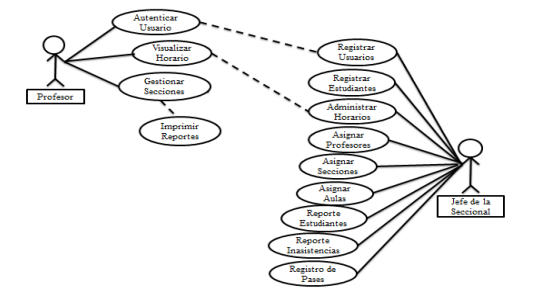
\includegraphics[width = 0.8\textwidth]{./figuras/estaticaMal.png}
\caption{Casos de uso.}
\label{fig:estMal}
\end{figure}

A pesar de que co visto na figura podese interpretar perfectamente a intención principal do software, podería realizarse o diagrama de unha forma mais detallada e explicita, explicando correctamente o tipo de relación entre os modulos (extension, inclusión...).

Por outro lado podería incluirse no documento unha descripción detallada dos modulos, cos cursos de acción dos casos de uso, pre e post condicions, cursos anómalos do proceso, etc.
\newpage
\subsubsection{Diagrama de clases}
\begin{figure}[h]
\centering
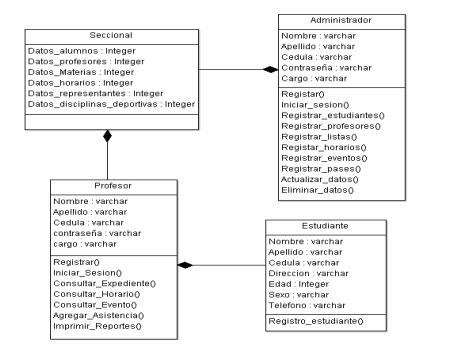
\includegraphics[width = 0.8\textwidth]{./figuras/clasesMal.png}
\caption{Diagrama de clases.}
\label{fig:clasesMal}
\end{figure}

Ó igual que nos casos de uso o diagrama de clases do documento da UETD \cite{UETD} resulta pouco especifico, sobre todo en canto á representación dos metodos, non temos forma de saber si son privados ou públicos por exemplo.
\newpage
\subsection{Vista dinámica}
A figura \ref{fig:dinMal} representa a vista dinámica pertencente ó sistema citado xa no caso anterior.\cite{UETD}
\begin{figure}[!h]
\centering
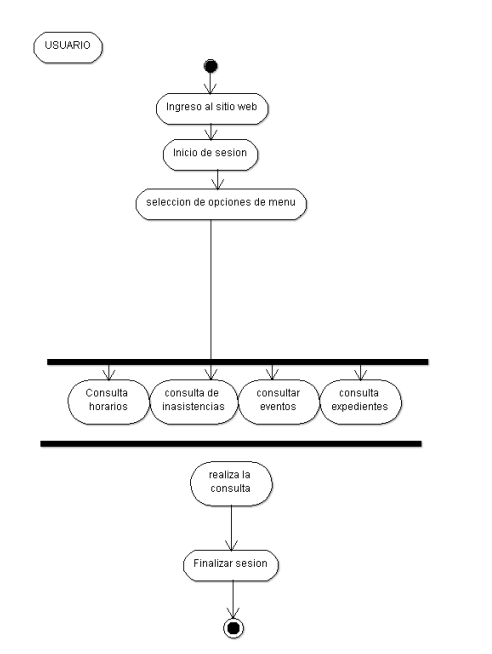
\includegraphics[width = 0.8\textwidth]{./figuras/dinamicaMal.png}
\caption{Vista Dinámica.}
\label{fig:dinMal}
\end{figure}

Ó igual que no caso anterior a representación é completamente comprensible dada a simpleza do sistema, sen embargo podería usarse unha notacion mais acorde cos estándares UML e IEE 1471, de esta forma representaríase unha sucesión de accions e as respostas dadas polo sistema en cada un dos módulos. Tendo en conta tanto o funcionamiento correcto como as posibles devolucions en caso de erro.

\subsection{Vista de despregue}\label{sec:despMal}
A continuación amosase unha imaxe dunha mala descripción da implementación dun sistema (\ref{fig:despMal}). O diagrama pertence a un sistema do módulo de Recursos Humanos para a divisiónde persoal da ENAHP-IUT.\cite{ENAHP}
\begin{figure}[h]
\centering
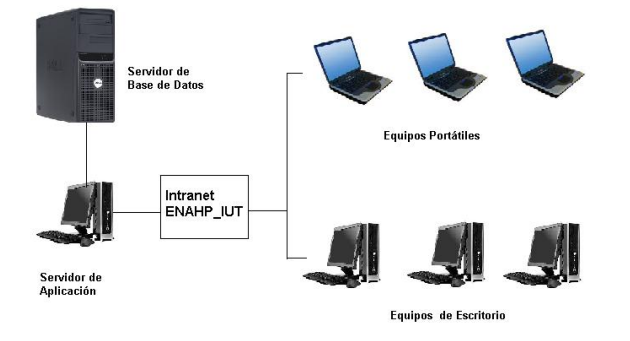
\includegraphics[width = 0.8\textwidth]{./figuras/despliegueMal.png}
\caption{Vista Despregue.}
\label{fig:despMal}
\end{figure}

Neste caso vemos unha representación fora dos cánones, na que non se especifica a tecnoloxía empregada en cada unha das partes nin para o procesado, nin para o manexo de comunicacións. Sen embargo cabe destacar que en outros apartados do documento si se fai mención a isto mediante unha representacion dun modelo de capas, a pesar disto esta parte do documento tampouco segue unha notación estandar.

\newpage
\section{Unha boa representación arquitectural}
\subsection{Vista estática}
\subsubsection{Casos de uso}
O analizar o documento tratado na seccion \ref{sec:despMal} vemos que a pesar de que ese diagrama non seña completo, no caso da descripción estática seguen unha boa metodoloxía con respecto os estandares (Ver fig. \ref{fig:estBien}).

Conxuntamente incluen unha descripción detallada de cada un dos modulos (Ver fig. \ref{fig:cu}), e os seus posibles comportamentos, o cal facilita en gran medida a comprensión do sistema por calquer analista ou programador que vexa o documento.\cite{ENAHP}
\begin{figure}[ht]
\centering
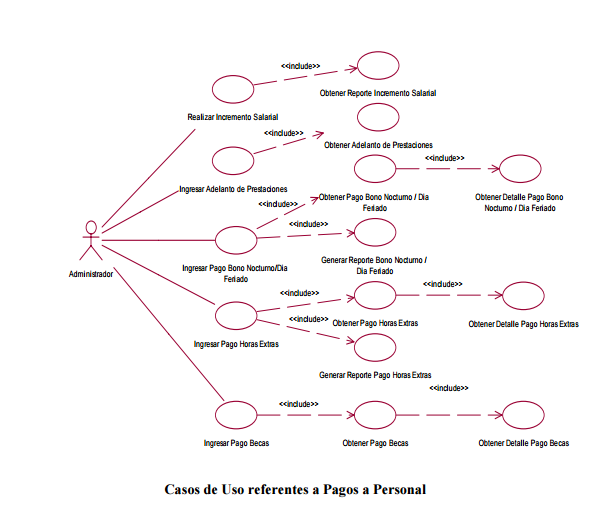
\includegraphics[width=0.8\textwidth]{./figuras/estaticaBien.png}
\caption{Casos de uso.}
\label{fig:estBien}
\end{figure}
\begin{figure}[h]
\centering
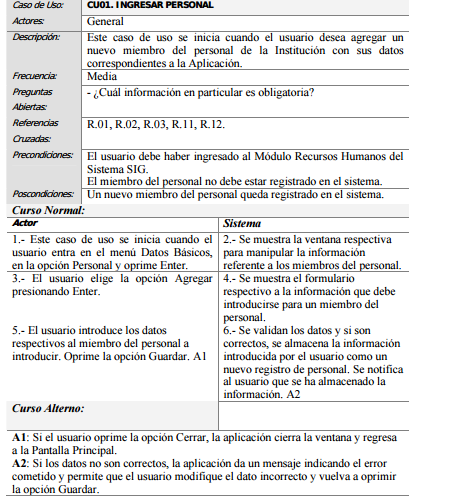
\includegraphics[width=0.8\textwidth]{./figuras/cu.png}
\caption{Caso de uso detallado.}
\label{fig:cu}
\end{figure}

\newpage
\subsubsection{Diagrama de clases}
No Documento anterior \cite{ENAHP} tamén se realizada unha exposición detallada do diagrama de clases, mediante varias figuras, a primeira (ver fig. \ref{fig:clasesBien}) que representa as relacións entre as clases de forma detallada e especifica, e varias representacións posteriores explicando os atributos e metodos de cada unha das clases (ver fig. \ref{fig:clasesBienDet}).

\begin{figure}[h]
\centering
\subfloat[Diagrama]{
\label{fig:clasesBien}
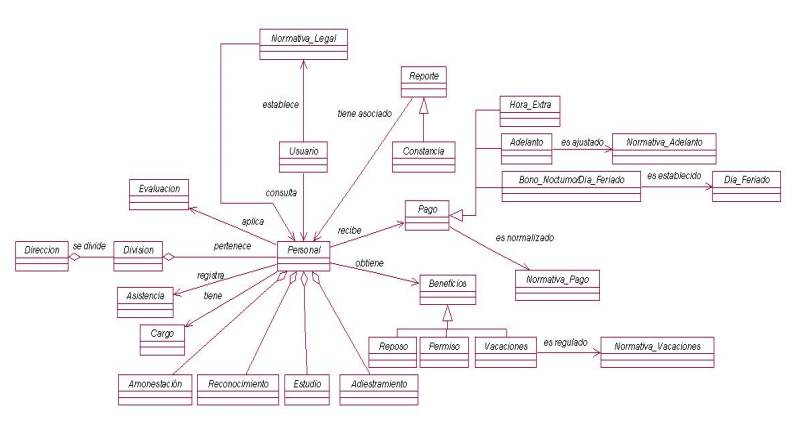
\includegraphics[width=40mm]{./figuras/clasesBien.png}}
\subfloat[Descripción]{
\label{fig:clasesBienDet}
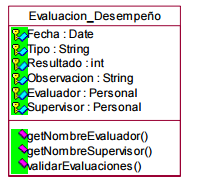
\includegraphics[width=40mm]{./figuras/clasesBienDesc.png}}
\caption{Diagrama de clases.}
\label{fig:clasesBienTot}
\end{figure}

\newpage
\subsection{Vista dinámica}
Analizando o documento de arquitectura software citado no apartado anterior \cite{ENAHP} vemos que os diagramas da vista dinámico están realizados de un xeito correcto, especifacando os actores a as partes do software involucrado, o tipo de comunicacions, e as posibles devolucións realizadas no proceso

\begin{figure}[h]
\centering
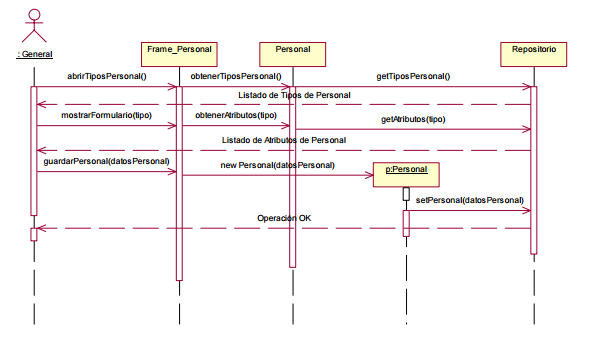
\includegraphics[width=0.8\textwidth]{./figuras/dinamicaBien.png}
\caption{Vista Dinámica.}
\label{fig:dinBien}
\end{figure}
\newpage
\subsection{Vista de despregue}

\section{Representación arquitectural do sistema-anel}

Realizarase a representación arquitectural do sistema-anel.

\subsection{Descomposición en módulos}
\subsubsection{Casos de uso}
O usuario interactuará có sistema a traves de tres tipos de operacións basicas como se ve na fig. \ref{fig:anelEstCU}

\begin{figure}[h]
\centering
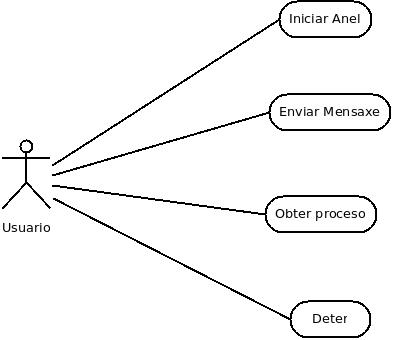
\includegraphics[width=0.8\textwidth]{./figuras/Diagrama1.jpeg}
\caption{Vista Estática, Casos de uso.}
\label{fig:anelEstCU}
\end{figure}

\paragraph{Iniciar Anel}
Neste módulo procederáse a crear un poceso "head" que se encargará de crear tantos procesos conectados entre sí, como indique o usuario.

Estos procesos iranse conectando entre eles formando unha topoloxía de anel.
\paragraph{Enviar Mensaxe}
O proceso "head" enviará unha mensaxe tantas mensaxes ó anel como o usuario especifique. Dentro do anel a mensaxe enviarase dun proceso o seguinto ata rematar a cadea.
\paragraph{Obter Proceso}
Trátase dunha función auxiliar que devolve o Pid do proceso que ocupe a posición no anel indicada polo usuario.
\paragraph{Deter}
O sistema para todos los procesos que se estean a executar.
\newpage
\subsubsection{Diagrama de clases}

\begin{figure}[h]
\centering
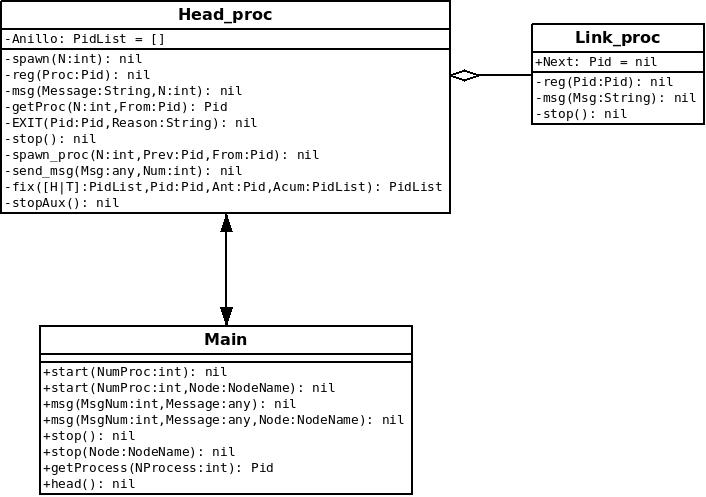
\includegraphics[width=0.8\textwidth]{./figuras/Diagrama2.jpeg}
\caption{Vista Estática, Casos de uso.}
\label{fig:anelEstCU}
\end{figure}

\subsection{Descomposición en procesos}


Todos os casos representados son nun escenario de un único nodo, en caso de haber envio de mensaxes entre nodos, habería que incluir o parámetro [nome de nodo] no contido da mensaxe.
\newpage
\subsubsection{Iniciar Anel}

\begin{figure}[h!]
\centering
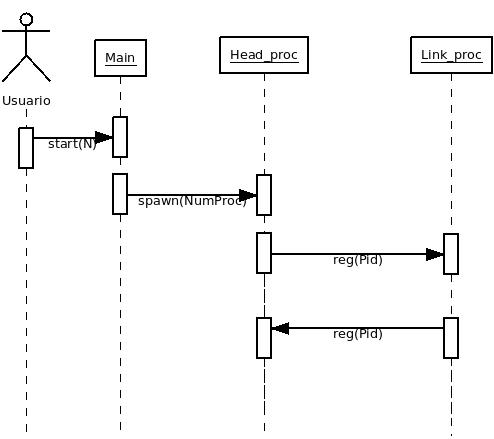
\includegraphics[width=0.8\textwidth]{./figuras/Diagrama3.jpeg}
\caption{Iniciar Anel.}
\label{fig:anelEstCU}
\end{figure}

\newpage
\subsubsection{Enviar Mensaxe}

\begin{figure}[h!]
\centering
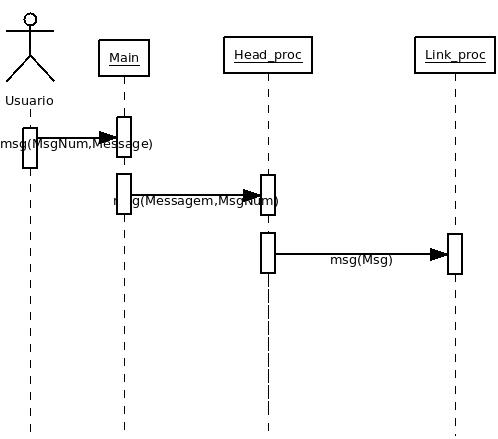
\includegraphics[width=0.8\textwidth]{./figuras/Diagrama4.jpeg}
\caption{Enviar Mensaxe.}
\label{fig:anelEstCU}
\end{figure}

\newpage
\subsubsection{Obter Proceso}

\begin{figure}[h]
\centering
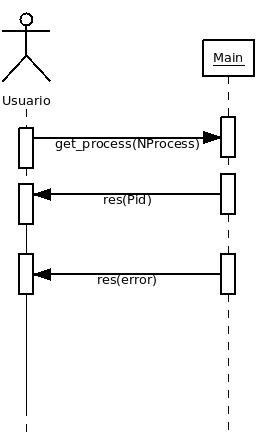
\includegraphics[width=0.5\textwidth]{./figuras/Diagrama5.jpeg}
\caption{Obter Proceso.}
\label{fig:anelEstCU}
\end{figure}

\newpage
\subsubsection{Deter}

\begin{figure}[h]
\centering
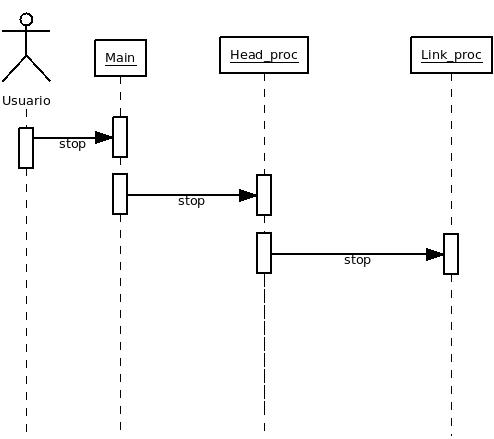
\includegraphics[width=0.8\textwidth]{./figuras/Diagrama6.jpeg}
\caption{Deter procesos.}
\label{fig:anelEstCU}
\end{figure}
\newpage
\subsection{Descomposición de despregue}

\begin{figure}[h]
\centering
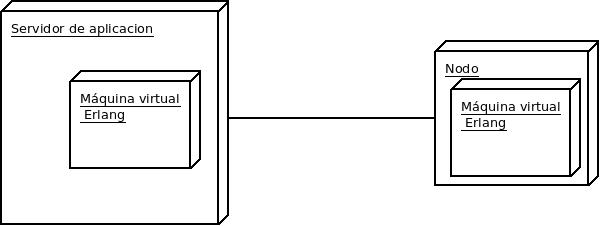
\includegraphics[width=0.8\textwidth]{./figuras/Diagrama7.jpeg}
\caption{Diagrama de despregue.}
\label{fig:despregue}
\end{figure}
\section{Bibliografía}
\begin{thebibliography}{2}
\bibitem{UETD} \textsc{Fernandez A., Hernández M.}
\textit{Desarrollo de un Sistema de Gestión para la Seccional de la U.E.T.D. "Liceo Caracas"}
\url{https://sistemagestionseccional.files.wordpress.com/2012/07/arquitectura-del-software.pdf}
\bibitem{ENAHP} \textsc{Roselyn C., Piñango D.}
\textit{Módulo Sig-RH}
\url{http://ldc.usb.ve/~ci3715/classes/Arquitectura.pdf}
\end{thebibliography}
\end{document}
